\documentclass[report.tex]{subfiles}
\begin{document}

\chapter{Related Work} % (fold)
\label{cha:related_work}

% ==============================================================================
% ==============================================================================

\section{Non-Local Boxes} % (fold)
\label{sec:non_local_boxes}
Non-local boxes are theoretical objects where multiple parties share some
correlation. The study of non-local boxes was introduced by physicists Sandu
Popescu and Daniel Rohrlich as part of their research non quantum non-locality.

Non-local boxes were introduced as a correlation that achieved the algebraic
maximum of 4 in the CHSH inequality by Clauser et al in addition to maintaining
non-signalling while doing so.

Consider a device with two ends, held by Alice and Bob. Each provides an
input (\(x\) and \(y)\), and observe the output produced by the box (\(a\) and
\(b)\). The box is defined by the probability distribution \(P(a,b | x,y)\) 
where \(a, b, x, y \in {0, 1}\). 

\begin{figure}[H]
  \centering
  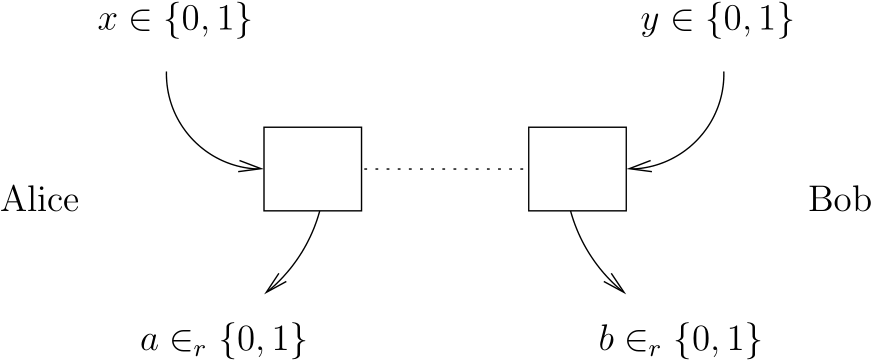
\includegraphics[width=0.66\textwidth]{img/nlb}
  \caption{A non local box}
\end{figure}

This device will immediately produce an output when given an input, preventing
any communication as a result of a delayed input. These devices are
non-signalling, ensuring that Alice cannot get any information about Bob's input
from her output, forbidding faster than light communication.
% subsubsection pr_box (end)

\subsection{Non-signalling} % (fold)
\label{sub:non_signalling}
As mentioned in Section \ref{sec:non_local_boxes}, an important part of the
non-local box is that it is non signalling. Non-signalling means that in the
described experiment, Alice can not be made aware of Bob's choice of input or
vice-versa. This requirement imposes restrictions on the probability
distribution, since the probability of an output should depend solely on its
respective input. 

The non-signalling restriction can be represented by the given formulae:
\[\sum_{b} P(a, b | x, y) = \sum_{b} P(a, b | x, y') = P(a | x) 
\quad \forall a, x, y, y'\]
\[\sum_{a} P(a, b | x, y) = \sum_{a} P(a, b | x', y) = P(b | y) 
\quad \forall b, y, x, x'\]

These restrictions allow for a definition of a reduced probability on the
outputs as well, \(P(a | x)\), which is useful information to have when
working with non-local boxes, especially as it pertains to creating models of
these boxes in PRISM, where the reduced probability is essential in the PRISM
model.
% subsection non_signalling (end)

\subsection{Example NLBs} % (fold)
\label{sub:example_nlbs}
Provided are some examples of standard non-local boxes. It is possible to have
non-local boxes with more than two inputs and outputs, and it is also possible
to have non-local boxes that handle a larger set of values than binary digits
as well. Note that for the tables below, the rows indicate input and the columns
indicate output.

\subsubsection{Classical Model} % (fold)
\label{ssub:classical_model}
The classical model is a simple example of a non-local box. In our theoretical
device, a coin is toss inside the device, and whatever result it gives is sent
as the output to Alice or Bob. This behaviour produces the following probability
distribution.

\begin{table}[H]
  \centering
  \begin{tabular}{l | c c c c}
      & 00 & 01 & 10 & 11 \\
      \hline
      00 & \(\frac{1}{2}\) & 0 & 0 & \(\frac{1}{2}\) \\
      01 & \(\frac{1}{2}\) & 0 & 0 & \(\frac{1}{2}\) \\
      10 & \(\frac{1}{2}\) & 0 & 0 & \(\frac{1}{2}\) \\
      11 & \(\frac{1}{2}\) & 0 & 0 & \(\frac{1}{2}\) \\
  \end{tabular}
  \caption{Probability Distribution}
  \label{tab:classical}
\end{table}

As you can see, this upholds the non-signalling requirement, since the
distribution shows that a change of one input cannot influence the output at the
other end of the device. 
% subsubsection classical_model (end)

\subsubsection{PR-Box} % (fold)
\label{ssub:pr_box}
The PR-box, originally proposed by and named after Popescu and Rohrlich, can be
considered the `Hello World' of non-local boxes. It is the most basic structure,
with two inputs and two outputs, and is the basis for this area of research.

The PR-Box has the following probability distribution:
\[
    P(a, b | x, y) = 
    \begin{cases}
        \frac{1}{2} & \quad a \text{ XOR } B = x \text{ AND } y \\
        0 & \quad \text{otherwise} \\
    \end{cases}
\]

This set-up can again be described using a matrix denoting the probabilities as
in \ref{ssub:classical_model}, although the above notation is commonly used in
papers related to quantum non-locality.

\begin{table}[H]
  \centering
\begin{tabular}{l | c c c c}
  & 00 & 01 & 10 & 11 \\
  \hline
  00 & \(\frac{1}{2}\) & 0 & 0 & \(\frac{1}{2}\) \\
  01 & \(\frac{1}{2}\) & 0 & 0 & \(\frac{1}{2}\) \\
  10 & \(\frac{1}{2}\) & 0 & 0 & \(\frac{1}{2}\) \\
  11 & 0 & \(\frac{1}{2}\) & \(\frac{1}{2}\) & 0 \\
\end{tabular}
  \caption{Probability Distribution}
  \label{tab:pr}
\end{table}
% subsection example_nlbs (end)
% section non_local_boxes (end)

% ==============================================================================

\section{PRISM} % (fold)
\label{sec:prism}
PRISM is a probabilistic model checking tool. It allows for
the modelling of systems which exhibit some random nature to them. Examples
include quantum cryptography or wireless networking protocols. Models as such
discrete-time Markov Chains can be created using the PRISM language, and
experiments can be ran using these models.

PRISM can be used for modelling non-local boxes (see here), although it's
weaknesses in doing so are the inspiration for this project.
% section prism (end)
% chapter related_work (end)

\newpage
\end{document}